\tikzset{graphical tensor/.style = {draw, inner sep=2pt, minimum size=0.35cm}}
\chapter{Graphical Notation}
Index notation for tensors can be quite messy, just consider a term like
\begin{equation}
    (\covariantDerivative{\beta} \covariantDerivative{\gamma} - \covariantDerivative{\gamma}\covariantDerivative{\beta}) V_\alpha = \tensor{R}{^\mu_{\alpha\beta\gamma}}V_\mu.
\end{equation}
Its difficult to tell what's going on with all of the indices.
The names of indices isn't important, as long as we keep track of which indices we sum over and which indices are free.
So in this example, we sum over \(\beta\), \(\gamma\), and \(\mu\) and \(\alpha\) is free.
The only other important property is upper and lower indices.

Graphical notation gives us a way to keep track of these things without having to give names to the indices and makes operations like contraction of indices very natural.
The general idea is we have an object, be it a scalar, vector, or higher order tensor, and we draw lines coming off it, either from the top or bottom, to represent indices.

Starting with the simplest object, a scalar, this has no indices and so no lines coming off it.
We draw it as a box with a label:
\begin{equation}\tikzsetnextfilename{graphical-notation-scalar}
    \varphi = \tikz[baseline=-1pt]{ \node[graphical tensor] {\(\varphi\)}; }\,.
\end{equation}
We could leave the label of and use differently shaped nodes to distinguish objects, but I prefer the label.

The next simplest object is a contravariant vector, this has a single upper index which we denote with a line connected to the top of the object going up:
\begin{equation}\tikzsetnextfilename{graphical-notation-contravariant}
    V^\mu = \tikz[baseline=-2pt]{ \node[graphical tensor] (V) {\(V\)}; \draw (V.north) -- ++ (0, 0.5); }\,.
\end{equation}
Similarly we can denote a covariant vector, with a single lower index, by drawing a line from the bottom of the object going down:
\begin{equation}\tikzsetnextfilename{graphical-notation-covariant}
    V_\mu = \tikz[baseline=-2pt]{ \node[graphical tensor] (V) {\(V\)}; \draw (V.south) -- ++ (0, -0.5); }\,.
\end{equation}

This generalises to arbitrary tensors.
For example a rank two tensor with two contravariant indices is given by
\begin{equation}\tikzsetnextfilename{graphical-notation-doubly-contravariant-tensor}
    T^{\mu\nu} = \tikz[baseline=-2pt]{ \node[graphical tensor] (T) {\(T\)}; \draw ($(T.north) - (0.1, 0)$) -- ++ (0, 0.5); \draw ($(T.north) + (0.1, 0)$) -- ++ (0, 0.5); }\,,
\end{equation}
and a rank two tensor with two covariant indices is given by
\begin{equation}\tikzsetnextfilename{graphical-notation-doubly-covariant-tensor}
    T_{\mu\nu} = \tikz[baseline=-2pt]{ \node[graphical tensor] (T) {\(T\)}; \draw ($(T.south) - (0.1, 0)$) -- ++ (0, -0.5); \draw ($(T.south) + (0.1, 0)$) -- ++ (0, -0.5); }\,.
\end{equation}
We can also represent a mixed tensor:
\begin{equation}\tikzsetnextfilename{graphical-notation-mixed-tensor}
    \tensor{T}{^\mu_\nu} = \tikz[baseline=-2pt]{ \node[graphical tensor] (T) {\(T\)}; \draw ($(T.north) - (0.1, 0)$) -- ++ (0, 0.5); \draw ($(T.south) + (0.1, 0)$) -- ++ (0, -0.5); }\,.
\end{equation}

Note that the order of the lines from left to right is important, a line which starts on the left should end on the left, unless the order of indices is swapped.
This allows us to represent transposition by crossing lines:
\begin{equation}
    (T^\top)^{\mu\nu} = T^{\nu\mu} \iff
    \tikzsetnextfilename{graphical-notation-transpose-tensor-1}
    \tikz[baseline=-2pt]{ \node[graphical tensor] (T) {\(T^\top\)}; \draw ($(T.north) - (0.1, 0)$) -- ++ (0, 0.5); \draw ($(T.north) + (0.1, 0)$) -- ++ (0, 0.5); }
    =
    \tikzsetnextfilename{graphical-notation-transpose-tensor-2}
    \tikz[baseline=-2pt]{ \node[graphical tensor] (T) {\(T\)}; \draw[rounded corners] ($(T.north) + (0.1, 0.04)$) -- ++ (0, 0.1) -- ++ (-0.2, 0.3) -- + (0, 0.092); \draw[white, ultra thick, rounded corners] ($(T.north) + (-0.1, 0.04)$) -- ++ (0, 0.1) -- ++ (0.2, 0.3) -- + (0, 0.092); \draw[rounded corners] ($(T.north) + (-0.1, 0.04)$) -- ++ (0, 0.1) -- ++ (0.2, 0.3) -- + (0, 0.092); }\,.
\end{equation}

The metric tensor and its inverse are represented by no box with two legs down or up, respectively:
\begin{equation}
    g_{\mu\nu} =
    \tikzsetnextfilename{graphical-notation-metric-lower}
    \tikz[baseline=(current bounding box)]{ \draw (0, 0) -- ++ (0, 0.3) arc (180:0:0.2) -- ++ (0, -0.3); } \,, \qqand g^{\mu\nu} =
    \tikzsetnextfilename{graphical-notation-metric-upper}
    \tikz[baseline=(current bounding box)]{ \draw (0, 0) -- ++ (0, -0.3) arc (0:-180:0.2) -- ++ (0, 0.3); } \,.
\end{equation}
The reason for this will become clear in a moment.

Contraction of indices is represented by joining the lines, for example the scalar product is
\begin{equation}\tikzsetnextfilename{graphical-notation-scalar-product}
    V^\mu U_\mu = \tikz[baseline = (current bounding box)]{ \node[graphical tensor] (V) at (0, 0) {\(V\)}; \node[graphical tensor] (U) at (0, 1) {\(U\)}; \draw (V) -- (U); }.
\end{equation}
We can also contract indices on the same object:
\begin{equation}\tikzsetnextfilename{graphical-notation-self-contraction}
    T^{\mu\mu} = \tikz[baseline=-3pt]{ \node[graphical tensor] (T) {\(T\)}; \draw ($(T.north) - (0.1, 0)$) -- ++ (0, 0.2) arc (180:0:0.1) -- ++ (0, -0.2); } \,.
\end{equation}

Using this we can write the lowering of indices as
\begin{equation}
    g_{\nu\mu}V^\mu = V_\nu \iff
    \tikzsetnextfilename{graphical-notation-lowering-index-1}
    \tikz[baseline=-2pt]{ \node[graphical tensor] (V) {\(V\)}; \draw (V.north) -- ++ (0, 0.2) arc (0:180:0.2) -- ++ (0, -0.8); }
    =
    \tikzsetnextfilename{graphical-notation-lowering-index-2}
    \tikz[baseline=-2pt]{ \node[graphical tensor] (V) {\(V\)}; \draw (V.south) -- ++ (0, -0.25); } \,.
\end{equation}
Notice how the metric tensor naturally blends in with the line and we can very easily see the way it lowers the index.
Similarly the inverse of the metric can be used to raise indices:
\begin{equation}
    g^{\nu\mu}V_\mu = V^\nu \iff
    \tikzsetnextfilename{graphical-notation-raising-index-1}
    \tikz[baseline=-2pt]{ \node[graphical tensor] (V) {\(V\)}; \draw (V.south) -- ++ (0, -0.2) arc (0:-180:0.2) -- ++ (0, 0.8); }
    =
    \tikzsetnextfilename{graphical-notation-raising-index-2}
    \tikz[baseline=-2pt]{ \node[graphical tensor] (V) {\(V\)}; \draw (V.north) -- ++ (0, 0.25); } \,.
\end{equation}

The covariant derivative of a quantity is represented by a circle or oval around that object with a line off the circle going downwards to represent the lower index of the covariant derivative:
\begin{equation}\tikzsetnextfilename{graphical-notation-covariant-derivative}
    \covariantDerivative{\nu} V^\mu =
    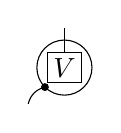
\begin{tikzpicture}[baseline=-2pt]
        \node[graphical tensor] (V) {\(V\)};
        \draw (V) -- ++ (0, 0.5);
        \draw (0, 0) circle [radius = 0.35];
        \fill (-135:0.35) circle [radius = 0.05];
        \draw (-135:0.35) to[bend right] (-135:0.65);
    \end{tikzpicture}
    \,.
\end{equation}
For example the Leibniz rule for the covariant derivative is given in graphical notation by
\begin{equation}
    \covariantDerivative{\nu} (V^\mu U^\rho) = (\covariantDerivative{\nu} V^\mu) U^\rho + V^\mu \covariantDerivative{\nu} U^\rho \iff
    \tikzsetnextfilename{graphical-notation-leibniz-1}
    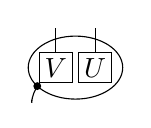
\begin{tikzpicture}[baseline=(current bounding box)]
        \node[graphical tensor] (V) {\(V\)};
        \draw (V) -- ++ (0, 0.5);
        \node[graphical tensor] (U) at (0.5, 0) {\(U\)};
        \draw (U) -- ++ (0, 0.5);
        \draw (0.25, 0) circle [x radius = 0.6, y radius = 0.4];
        \fill (-0.235, -0.235) circle [radius = 0.05];
        \draw[rounded corners] (-0.235, -0.235) -- ++ (-135:0.1) -- ++ (0, -0.1);
    \end{tikzpicture}
    =
    \tikzsetnextfilename{graphical-notation-leibniz-2}
    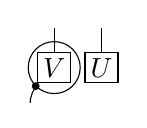
\begin{tikzpicture}[baseline=(current bounding box)]
        \node[graphical tensor] (V) {\(V\)};
        \draw (V) -- ++ (0, 0.5);
        \node[graphical tensor] (U) at (0.6, 0) {\(U\)};
        \draw (U) -- ++ (0, 0.5);
        \draw (0, 0) circle [radius = 0.33];
        \fill (-0.235, -0.235) circle [radius = 0.05];
        \draw[rounded corners] (-0.235, -0.235) -- ++ (-135:0.1) -- ++ (0, -0.1);
    \end{tikzpicture}
    +
    \tikzsetnextfilename{graphical-notation-leibniz-3}
    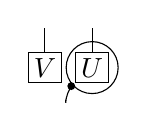
\begin{tikzpicture}[baseline=(current bounding box)]
        \node[graphical tensor] (V) {\(V\)};
        \draw (V) -- ++ (0, 0.5);
        \node[graphical tensor] (U) at (0.6, 0) {\(U\)};
        \draw (U) -- ++ (0, 0.5);
        \draw (0.6, 0) circle [radius = 0.33];
        \fill (0.335, -0.235) circle [radius = 0.05];
        \draw[rounded corners] (0.335, -0.235) -- ++ (-135:0.1) -- ++ (0, -0.1);
    \end{tikzpicture}
\end{equation}

At the start of this section we complained about the complexity of the statement
\begin{equation}
    (\covariantDerivative{\beta}\covariantDerivative{\gamma} - \covariantDerivative{\gamma}\covariantDerivative{\beta})V_\alpha = \tensor{R}{^\mu_{\alpha\beta\gamma}}V_\mu.
\end{equation}
We can simplify this equation slightly by introducing the concepts of symmetrisation and antisymmetrisation of indices.
This is were we write a set of indices once and implicitly sum over them in a way that makes the result either symmetric or antisymmetric in these indices.
Formally given some tensor \(T^{i_1i_2\dotso i_n}\) we define the symmetrisation of the indices to be
\begin{equation}
    T^{(i_1i_2\dotso i_n)} \coloneqq \frac{1}{n!}\sum_{\sigma \in S_n} T^{\sigma(i_1)\sigma(i_2) \dotso \sigma(i_n)}
\end{equation}
where \(S_n \coloneqq \{\sigma \colon \{1, \dotsc, n\} \to \{1, \dotsc, n\} \mid \sigma \text{ is a bijection}\}\) is the permutation group\footnote{See the notes from the symmetries of quantum mechanics course.}.
Any indices outside the brackets are ignored
For example,
\begin{equation}
    T^{(ij)k} = \frac{1}{2}(T^{ijk} + T^{jik}),
\end{equation}
and
\begin{equation}
    T^{(ijk)} = \frac{1}{3!} (T^{ijk} + T^{ikj} + T^{jki} + T^{jik} + T^{kij} + T^{kji}).
\end{equation}
Similarly the antisymmetrisation is defined by
\begin{equation}
    T^{[i_1i_2\dotso i_n]} \coloneqq \frac{1}{n!}\sum_{\sigma \in S_n} \sgn(\sigma) T^{\sigma(i_1)\sigma(i_2)\dotso \sigma(i_n)}
\end{equation}
where \(\sgn(\sigma)\) is \(+1\) for an even permutation and \(-1\) for an odd permutation.
For example,
\begin{equation}
    T^{[ij]k} = \frac{1}{2}(T^{ijk} - T^{jik}),
\end{equation}
and
\begin{equation}
    T^{[ijk]} = \frac{1}{3!}(T^{ijk} - T^{ikj} + T^{jki} - T^{jik} + T^{kij} - T^{kji}).
\end{equation}

It is possible to (anti)symmetrise over indices on different objects.
For example,
\begin{equation}
    V^{(\mu}U^{\nu)} = \frac{1}{2}(V^\mu U^\nu + V^\nu U^\mu), \qqand V^{[\mu}U^{\nu]} = \frac{1}{2}(V^\mu U^\nu - V^\nu U^\mu).
\end{equation}

Using antisymmetrisation of indices we can write the complex statement from the start as
\begin{equation}
    2\covariantDerivative{[\beta}\covariantDerivative{\gamma]} V_\alpha = \tensor{R}{^\mu_{\alpha\beta\gamma}}V_\mu.
\end{equation}

The graphical notation for symmetrising indices is to put a thick zig zag across the indices.
The factor of \(1/n!\), if present, is explicitly written.
So
\begin{equation}
    T^{(ij)} = \frac{1}{2}(T^{ij} + T^{ji}) \iff 2
    \tikzsetnextfilename{graphical-notation-symmetrisation-1}
    \tikz[baseline=-3pt]{ \node[graphical tensor] (T) {\(T\)}; \draw ($(T.north) + (-0.1, 0)$) -- ++ (0, 0.6); \draw ($(T.north) + (0.1, 0)$) -- ++ (0, 0.6); \draw[decoration={zigzag, segment length=5pt, pre length=1pt}, ultra thick, decorate] (-0.25, 0.5) -- ++ (0.5, 0); }
    \, = \,
    \tikzsetnextfilename{graphical-notation-symmetrisation-2}
    \tikz[baseline=-3pt]{ \node[graphical tensor] (T) {\(T\)}; \draw ($(T.north) + (-0.1, 0)$) -- ++ (0, 0.6); \draw ($(T.north) + (0.1, 0)$) -- ++ (0, 0.6); }
    +
    \tikzsetnextfilename{graphical-notation-symmetrisation-3}
    \tikz[baseline=-3pt]{ \node[graphical tensor] (T) {\(T\)}; \draw[rounded corners] ($(T.north) + (0.1, 0.04)$) -- ++ (0, 0.1) -- ++ (-0.2, 0.3) -- + (0, 0.092); \draw[white, ultra thick, rounded corners] ($(T.north) + (-0.1, 0.04)$) -- ++ (0, 0.1) -- ++ (0.2, 0.3) -- + (0, 0.092); \draw[rounded corners] ($(T.north) + (-0.1, 0.04)$) -- ++ (0, 0.1) -- ++ (0.2, 0.3) -- + (0, 0.092); }
\end{equation}
Antisymmetrisation is written with a thick line across the indices:
\begin{equation}
    T^{(ij)} = \frac{1}{2}(T^{ij} + T^{ji}) \iff 2
    \tikzsetnextfilename{graphical-notation-antisymmetrisation-1}
    \tikz[baseline=-3pt]{ \node[graphical tensor] (T) {\(T\)}; \draw ($(T.north) + (-0.1, 0)$) -- ++ (0, 0.6); \draw ($(T.north) + (0.1, 0)$) -- ++ (0, 0.6); \draw[ultra thick] (-0.25, 0.5) -- ++ (0.5, 0); }
    \, = \,
    \tikzsetnextfilename{graphical-notation-antisymmetrisation-2}
    \tikz[baseline=-3pt]{ \node[graphical tensor] (T) {\(T\)}; \draw ($(T.north) + (-0.1, 0)$) -- ++ (0, 0.6); \draw ($(T.north) + (0.1, 0)$) -- ++ (0, 0.6); }
    -
    \tikzsetnextfilename{graphical-notation-antisymmetrisation-3}
    \tikz[baseline=-3pt]{ \node[graphical tensor] (T) {\(T\)}; \draw[rounded corners] ($(T.north) + (0.1, 0.04)$) -- ++ (0, 0.1) -- ++ (-0.2, 0.3) -- + (0, 0.092); \draw[white, ultra thick, rounded corners] ($(T.north) + (-0.1, 0.04)$) -- ++ (0, 0.1) -- ++ (0.2, 0.3) -- + (0, 0.092); \draw[rounded corners] ($(T.north) + (-0.1, 0.04)$) -- ++ (0, 0.1) -- ++ (0.2, 0.3) -- + (0, 0.092); }
\end{equation}
So the complex equation we started with can be expressed as
\begin{equation}
    (\covariantDerivative{\beta}\covariantDerivative{\gamma} - \covariantDerivative{\gamma}\covariantDerivative{\beta})V_\alpha = \tensor{R}{^\mu_{\alpha\beta\gamma}}V_\mu \iff
    \tikzsetnextfilename{graphical-notation-ricci-identity-1}
    \tikz[baseline=-0.1cm]{ \node[graphical tensor] (V) {\(V\)}; \draw (V.south) -- ++ (0, -0.5); \draw (V) circle [radius = 0.35]; \draw (V) circle [radius = 0.5]; \fill (-135:0.35) circle [radius = 0.05]; \fill (-135:0.5) circle [radius = 0.05]; \draw (-135:0.35) arc (90:180:0.5) -- ++ (0, -0.1); \draw (-135:0.5) arc (90:180:0.3) -- ++ (0, -0.2); \draw[ultra thick] (-0.85, -0.7) -- ++ (0.3, 0); }
    \, = \,
    \tikzsetnextfilename{graphical-notation-ricci-identity-2}
    \tikz[baseline=-0.1cm]{
        \node[graphical tensor, minimum width=0.8cm] (R) {\(R\)};
        \draw ($(R.south) + (0.3, 0)$) -- ++ (0, -0.1) arc (0:-90:0.1) arc (90:180:0.1) -- ++ (0, -0.2);
        \draw ($(R.south) + (0.1, 0)$) -- ++ (0, -0.1) arc (0:-90:0.1) arc (90:180:0.1) -- ++ (0, -0.2);
        \draw[ultra thick, white] ($(R.south) - (0.1, 0)$) -- ++ (0, -0.1) arc (-180:-90:0.1) -- ++ (0.2, 0) arc (90:0:0.1) -- ++ (0, -0.2);
        \draw ($(R.south) - (0.1, 0)$) -- ++ (0, -0.1) arc (-180:-90:0.1) -- ++ (0.2, 0) arc (90:0:0.1) -- ++ (0, -0.2);
        \node[graphical tensor] (V) at ($(R) + (1, 0)$) {\(V\)};
        \draw ($(R.north) - (0.3, 0)$) -- ++ (0, 0.3) arc (180:90:0.2) -- ++ (0.9, 0) arc (90:0:0.2) -- (V.north); }
\end{equation}
Note that the crossing over of the lines is the same complexity as the index order in this equation, on the left hand side the indices appear in the order \(\beta\), \(\gamma\), \(\alpha\), whereas on the right hand side they appear in the order \(\alpha\), \(\beta\), \(\gamma\).